% !TEX root = ../../main.tex

\section{Energetics of adsorption}

\subsection{Forces involved in adsorption}

From a classical molecular point of view, we can define the 
guest-host and guest-guest interactions as a sum of several
components with distinct physical meaning.

\begin{equation}\label{calo:eqn:interactions}
  \Phi_t = \Phi_{R} + \Phi_{D} + \Phi_{C} + \Phi_{I}
\end{equation}

The first two types of interaction, namely short range 
electrostatic repulsion between the electron clouds of 
neighbouring atoms and long range dispersion arising from
incidental short-lived partial charges are common to all
atoms, and can therefore be called ``non-specific''. Such 
interactions are commonly modelled through the use of a 
Lennard-Jones type potential function.

\begin{equation}\label{calo:eqn:lennard-jones}
  V_\text{LJ} = 4\varepsilon \left[ \left(\frac{\sigma}{r}\right)^{12} - \left(\frac{\sigma}{r}\right)^6 \right]
\end{equation}

The latter two types, Coulombic interactions and induction 
interactions arise from permanent charges and multipoles in the 
system. Coulombic interactions are attraction and repulsion
interactions between charges such as molecular ions,
Induction, also known as polarization or Debye forces, is the interaction
between a charged particle or a multipole with the induced multipole
in a non-charged system. The ease of inducing such an interaction
in a molecule is termed polarizability. These interactions 
can be referred to as ``non-specific''.

The total interactions can also be broken down as contributions
from guest-host interactions and guest-guest interactions.
If changes in the adsorbent occur as a result of adsorption,
a host-host or self-potential interaction should be considered.
The guest-host interaction can be assumed constant for a homogeneous
surface or a function of coverage, in the case of a 
heterogeneous surface.

Unfortunately, only the total sum of all interactions
is measurable through direct methods. Therefore, the 
absolute contribution of each component is unknowable unless
computational methods are employed.

\subsection{Adsorption thermodynamics}

As mentioned in the previous section, adsorption 
is a consequence of intermolecular attraction between the 
material surface and the molecules of the fluid. The sum of 
all interactions accounts for the depth of the potential 
well and therefore for the energy corresponding to the 
process. As this energy is net positive, adsorption is an
overall exothermic phenomenon.

However, in order to make the transition from a molecular 
viewpoint to a macroscale bulk fluid representation of 
adsorption, the a thermodynamic description of the adsorbed 
phase of the process must be defined.

\subsection{The Gibbs surface excess approach}

A description of the adsorbed phase can be made through 
an expressing the change in density or concentration of fluid
from the adsorbent surface to the bulk phase. The density 
has a maxima in the immediate zone close to the surface, and then
decreases until it reaches the density of the bulk fluid.
However, when defined as such, the boundary between the 
two phases is difficult to pinpoint.
Therefore, in most cases it is useful to employ the concept 
of the Gibbs dividing surface.

\begin{figure}[htb]
  \centering

  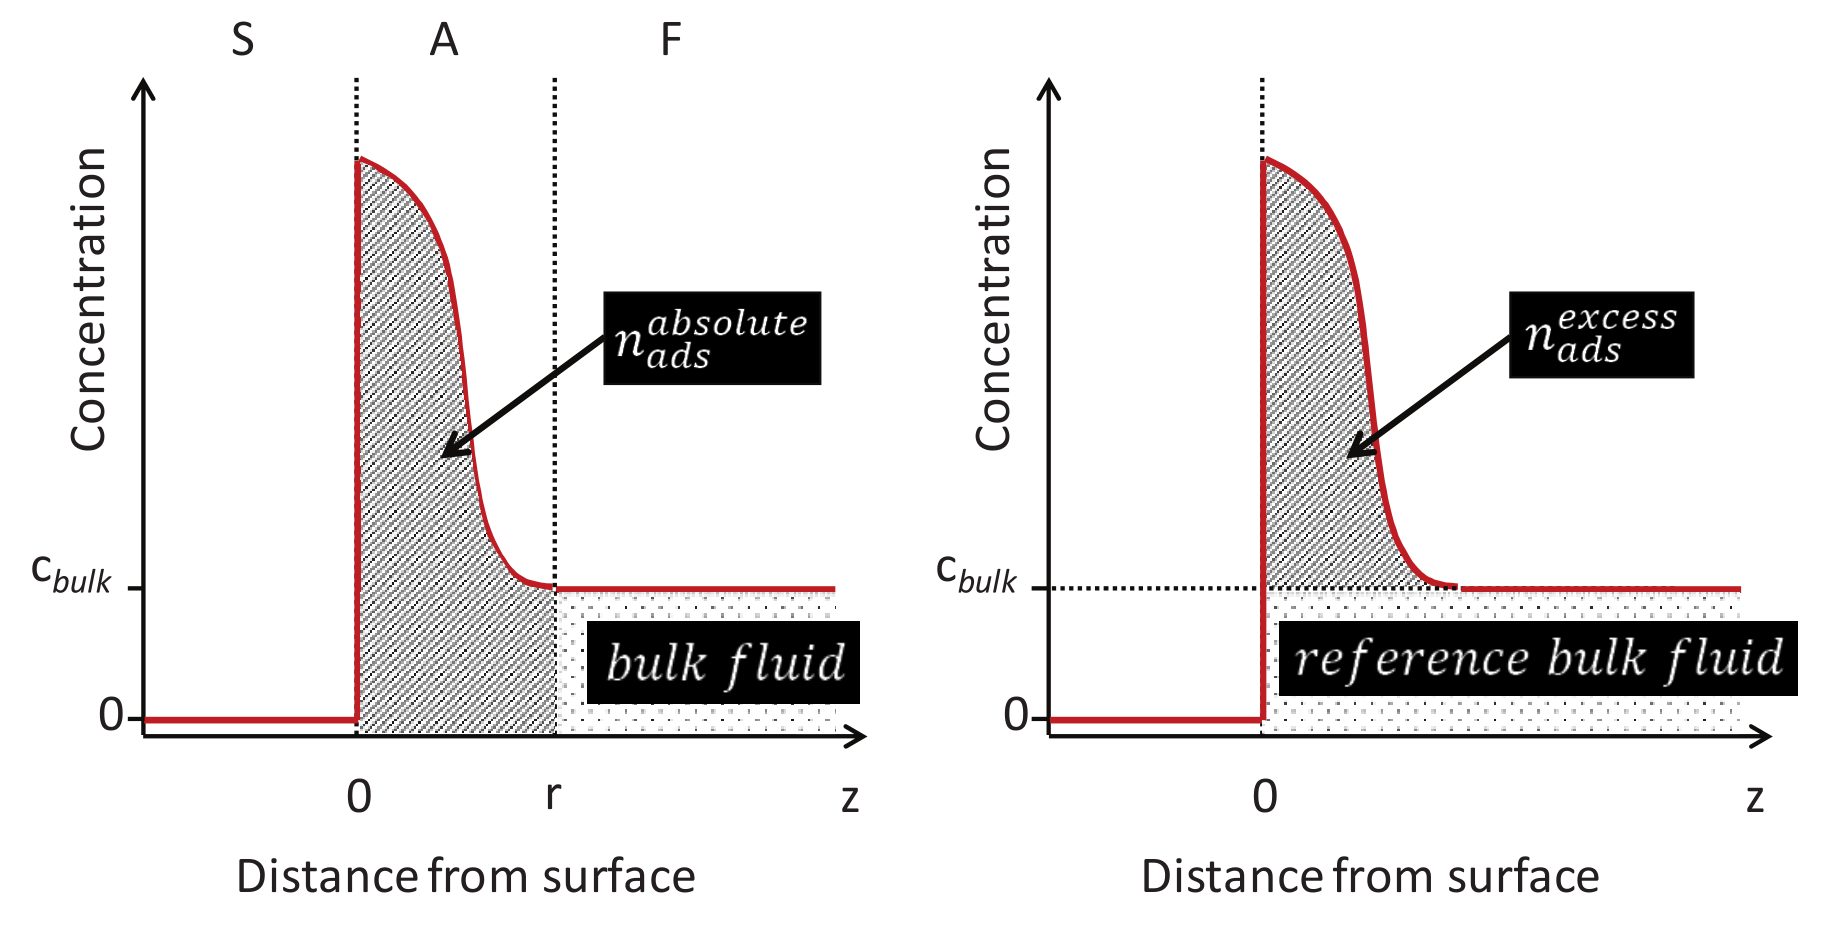
\includegraphics[width=\linewidth]{gibbs-surface}
  \caption{
    Representation of the adsorbed and bulk phases according to
    the (left) layer model and the (right) Gibbs dividing surface
    approach. Adapted from \citeauthor{rouquerolAdsorptionPowdersPorous2013}%
    \cite{rouquerolAdsorptionPowdersPorous2013}.
  }%
  \label{calo:fig:gibbs-surface}

\end{figure}

This approach describes the adsorbed phase only in terms
of an \textit{excess} from the properties of the bulk phase.
As represented in \autoref{calo:fig:gibbs-surface}, the total
amount adsorbed can be defined as:

\begin{equation}
  n_{ads}^{absolute} = A \int_0^r c\ dz
\end{equation}

The imaginary Gibbs dividing surface is placed such that the
concentration of the adsorbent in the adsorbed phase is only
measured as an excess from the concentration of the bulk fluid.
The relationship between the total amount adsorbed and the 
excess amount adsorbed is expressed as:

\begin{equation}
  n_{ads}^{excess} = n_{ads}^{absolute} + V_{ads} \cdot c_{bulk}
\end{equation}

As long as the volume of the adsorbed layer \(V_{ads}\) can be 
considered negligible and the concentration of adsorbate in the bulk 
phase \(c_{bulk}\) is low, the total amount adsorbed and the surface 
excess amount may be considered as approximately equal. 
At high pressures or when the difference in concentration between
the adsorbed and the bulk phase is low, the total amount adsorbed
begins to diverge significantly from the surface excess. 

Without corrections, both the gravimetric and manometric
method of adsorption will measure excess amounts adsorbed.
In the case of adsorption in porous materials, the volume of the
adsorbed phase may be taken as total pore volume. 

\subsection{Enthalpy of adsorption}

Adsorption can be considered as a closed system of constant volume
V and temperature T. No mass of material crosses the system boundary,
therefore the change in chemical potential is also
zero \(d\mu = 0\). The Helmholtz free energy is used for a description 
of the thermodynamic potential of such as system. 

The differential enthalpy of adsorption is then the change of the 
total enthalpy with respect to the number of moles adsorbed
at a certain equilibrium pressure and surface concentration.
It is given by:

\begin{equation}
  \Delta_{ads} \dot{h} = 
\end{equation}

The differential enthalpy of adsorption is often represented as a
function of partial coverage. In \autoref{calo:fig:enthalpy-iupac-iso},
isotherm types as defined by IUPAC are presented together with
a typical differential enthalpy curve. Type I isotherms often 
have an initial plateau, corresponding to adsorption in micropores
until a sharp decrease at complete pore filling occurs. If the surface
of the pores is heterogeneous, higher energy sites will be occupied
first, resulting in a sharp slope at low loadings. Multilayer
adsorption in non-porous or mesoporous materials (II and IV) yields
a slowly decreasing enthalpy curve, as the solid-guest interactions
drop off with increasing layers adsorbed. Finally, cooperative adsorption,
as seen in a type III isotherm, often gives rise to initial enthalpies
of adsorption which are below the enthalpy of vaporisation.
It should be noted that changes in the adsorbed fluid similar 
to phase changes may occur, which can be seen in the enthalpy curve
as a distinct peak~\cite{llewellynAdsorptionMFItypeZeolites1993, %
llewellynAdsorptionMFItypeZeolites1993a}.

\begin{figure}[htb]
  \centering

  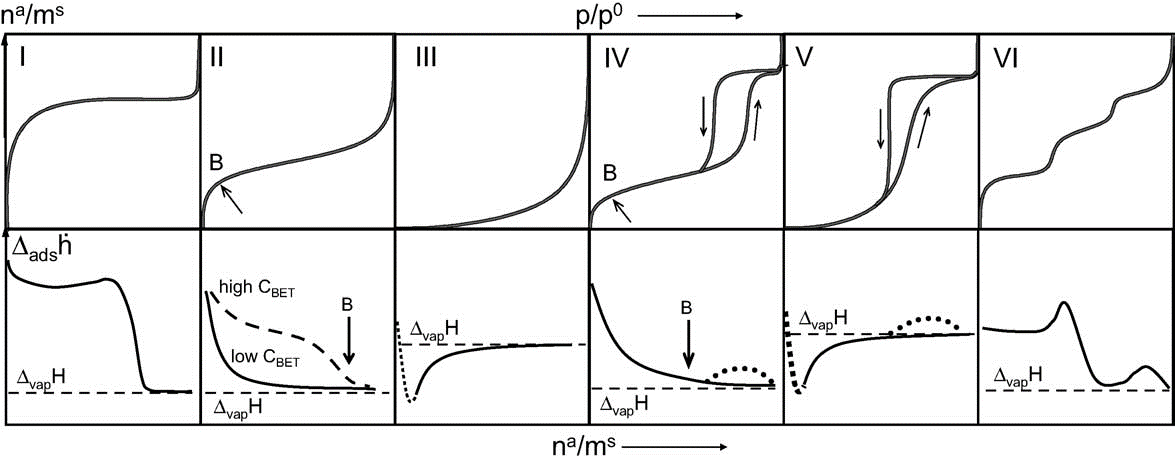
\includegraphics[width=\linewidth]{enthalpy-curves}
  \caption{
    Generalized curves of differential enthalpy of adsorption with 
    respect to coverage corresponding to different 
    IUPAC-defined isotherm types.
    Adapted from \citeauthor{llewellynGasAdsorptionMicrocalorimetry2005}%
    \cite{llewellynGasAdsorptionMicrocalorimetry2005}.
  }%
  \label{calo:fig:enthalpy-iupac-iso}

\end{figure}

\subsection{Measuring the enthalpy of adsorption}

Experimentally, two methods are widely used for determining the 
enthalpy of adsorption. The first relies on the applicability of the 
Clausius-Clapeyron equation to two or more isotherms measured 
at different temperatures while the second is a 
direct measurement of the evolved heat during adsorption 
using calorimetry.

A value for the enthalpy of adsorption in a particular system
may also be obtained from computer simulation methods. 
The accuracy of these procedures depends on the accuracy of
the chosen model of interaction between simulated molecules.

\subsubsection{Isosteric enthalpy of adsorption}

The isosteric enthalpy of adsorption is calculated from experimental
data using the Clausius-Clapeyron equation as the starting point:

\begin{equation}
    \Big( \frac{\partial \ln P}{\partial T} \Big)_{n_a} = -\frac{\Delta H_{ads}}{R T^2}
\end{equation}

Where \(\Delta H_{ads}\) is the isosteric enthalpy of adsorption.
If it is assumed that the adsorption enthalpy does not vary with 
temperature, the equation can be rearranged to:

\begin{equation}
    \Delta H_{ads} = - R \frac{\partial \ln P}{\partial 1 / T}
\end{equation}

In order to approximate the partial differential, two or more
isotherms are measured at different temperatures. 
Afterwards the isosteric enthalpy of adsorption can be calculated
by using the pressures at which the loading is identical using the 
rearranged equation. By plotting the values of \(\ln P\) against
\(1 / T\) we should obtain a straight line with a slope
of \(- \Delta H_{ads} / R\).

The isosteric enthalpy is sensitive to the differences in pressure between
the two isotherms. If the isotherms measured are too close together, 
the error margin will increase. The method also assumes that isosteric
enthalpy does not vary with temperature. If the
variation is large for the system in question, the calculation will
give unrealistic values.

Even with carefully measured experimental data, there are two 
assumptions used in deriving the Clausius-Clapeyron equation: 
an ideal bulk gas phase and a negligible adsorbed phase
molar volume. These have a significant effect on the calculated 
isosteric enthalpy of adsorption, especially at high relative pressures 
and for heavy adsorbates.

\subsubsection{Microcalorimetry}

A direct measurement of the enthalpy of adsorption is possible using
calorimetric methods.

The 
For the best performance, a 3D Tian-Calvet thermopile is used, which
allows for a complete integration of evolved heat.

Two options exist, based on two methods of obtaining adsorption isotherms:
the continuous and the discontinuous or point-by-point method. In
the point-by-point method, discrete steps of introduction of adsorbate 
are taken. A reference volume is filled with gas at a pressure p, which
is allowed to equilibrate before a valve between the reference volume 
and the cell containing the adsorbate. 
In the other method, the flow of adsorbate is continuous, usually kept 
constant by a restriction in the pipe diameter which is severe enough
to enter sonic flow regimes. At this point, the flowrate is no longer 
influenced by a pressure differential, instead becoming a function only
of upstream pressure and environment temperature.

The heat generated during adsorption (or required during desorption)
is therefore measured either as discrete peaks, corresponding to 
each event or as a continuous heat curve. An example of such a signal 
is presented in \todo{figure}.

The point-by-point method is less accurate than a continuous introduction,
as the measured heat is necessarily a cumulative value of instantaneous
differential enthalpy for the coverage range of each adsorbed point.
However, it has the advantage of ensuring complete equilibrium at 
each step, by observing the return to the baseline of the calorimetry
signal, or no changes in the pressure signal. On the other hand, the 
continuous method allows for subtle changes in the enthalpy of 
adsorption, such as those corresponding to adsorbed phase ordering or 
changes, to be seen experimentally. Additionally, the time-resolved data
can be used to investigate transient phenomena. Equilibrium between 
the adsorbed phase and gas phase is no longer assured, and must be
tested for by performing multiple experiments at different adsorbate
flowrates. Alternatively, the experiment can be stopped to observe that the 
time for the heat signal to return to its baseline does not diverge 
from the dead time of the calorimeter.

The heat value which is measured through calorimetry corresponds to 
two components, the differential enthalpy of adsorption and the 
work required to expand the gas into the measurement cell.
In this relationship as expressed in \autoref{calo:eqn:calo-heat}
the value for work can be substituted by \(V\Delta P\) and 
accounted for at each point.

\begin{align}\
  \dot{Q} & = \Delta_{ads} h + W \label{calo:eqn:calo-heat} \\
  \dot{Q} & = \Delta_{ads} h + V\Delta P \\
  \Delta_{ads} h & = \dot{Q} - V\Delta P
\end{align}

Finally, to obtain a value for the differential enthalpy of adsorption,
the enthalpy is divided by the amount of gas adsorbed in the same 
time.